\documentclass{article}
\usepackage[brazil]{babel}
\usepackage[utf8]{inputenc}
\usepackage{indentfirst}
\usepackage[T1]{fontenc}
\usepackage{gensymb}
\usepackage{graphicx}
\usepackage{etoolbox}
\usepackage{listings}
\usepackage[a4paper, left=20mm, right=20mm, top=20mm, bottom=20mm]{geometry}
\usepackage[colorlinks, urlcolor=blue, citecolor=red]{hyperref}



\begin{document}

\title{\textbf{Neural Network}}
\author{
    Lucas Ribeiro Neis\\
     {\texttt{lucasrneis@gmail.com}}
     \and
     Vinícius Couto Biermann\\
      {\texttt{viniciusbiermann@hotmail.com}}
      \vspace{-50mm}
}
\date{Novembro 2016}

\maketitle

\section{Introdução}
Foi proposto um trabalho para reconhecimento de dígitos manuscritos utilizando o conhecimento adquirido de redes neurais. Foi disponibilizado o arquivo \texttt{exdata.m} contendo dados obtidos a partir de um subconjunto da base de dados MNIST.
Foi escolhida a ferramente \texttt{MATLAB} para a realização do trabalho.

\section{Desenvolvimento}

A normalização dos dados foi feita usando o comando mapminmax.\\
\hspace*{2cm} $[inTrain\_N,PS]=mapminmax(inTrain);$ 
\newline

Inicialmente, separamos o conjunto de entradas em dois conjuntos, um para testes e outro para treinamento. Mas, após alguns testes, alteramos para apenas um conjunto separando-o através do uso de parâmetros:

\begin{lstlisting}[mathescape]
    net.divideParam.trainRatio=0.7;
    net.divideParam.valRatio=0.0;
    net.divideParam.testRatio=0.3;
\end{lstlisting}

A ausência de validação deve-se que conseguimos melhores resultados sem ela.

Além disso, testamos diversos algoritmos e combinações de números de camadas com diversas funções. Conseguimos resultados safisfatórios com \texttt{Conjugate Gradient with Beale-Powell Restars} (ou \texttt{traincgb} no \texttt{MATLAB}) como mostrado na figura \ref{fig0}. Infelizmente, não conseguimos usar \texttt{Levenberg-Marquardt} devido a problemas com a execução.

\begin{figure}[h!]
    \centering
    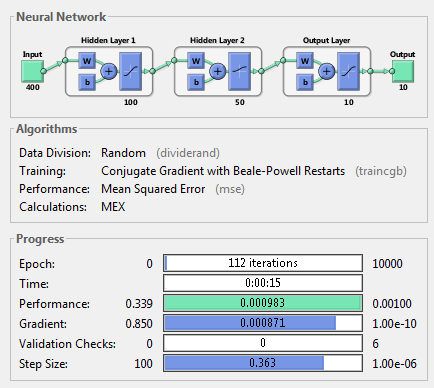
\includegraphics[scale=0.7]{fig0.png}
    \caption{Exemplo de uma tela de testes.}
    \label{fig0}
\end{figure}

Como mostra a figura \ref{fig1}, usamos duas camadas escondidas:
\begin{itemize} \setlength{\itemindent}{1cm}
    \item \texttt{Hidden Layer 1:}
    São cem neurônios usando \texttt{tansig}.
    \item \texttt{Hidden Layer 2:}
    São cinquenta neurônios usando \texttt{logsig}.
\end{itemize}

Além disso, a camada de saída tem os 10 neurônios por padrão e usa \texttt{tansig} como funções de saída.

\begin{figure}[h!]
    \centering
    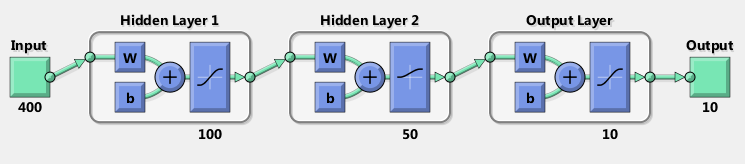
\includegraphics[scale=0.7]{fig1.png}
    \caption{Arquitetura da rede utilizada.}
    \label{fig1}
\end{figure}

\begin{figure}[h!]
    \centering
    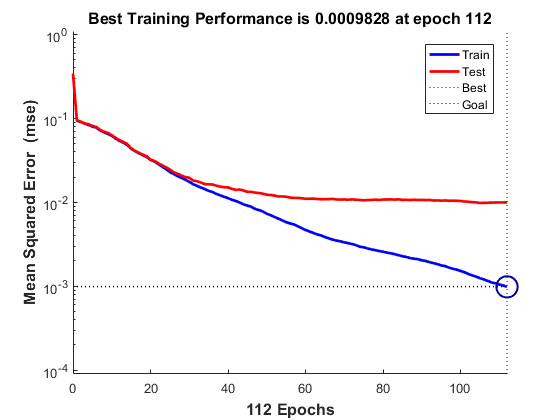
\includegraphics[scale=0.7]{fig2.png}
    \caption{Gráfico de performance no treinamento e teste.}
    \label{fig2}
\end{figure}

\begin{figure}[h!]
    \centering
    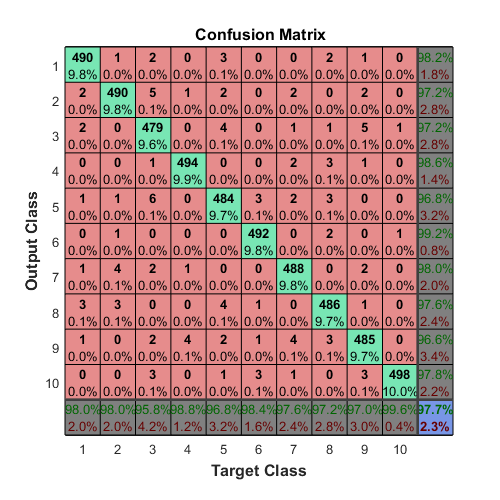
\includegraphics[scale=0.7]{fig3.png}
    \caption{Matriz de confusão obtida.}
    \label{fig3}
\end{figure}


\end{document}
